\section{Appendix}
\subsection{Class diagram}
\includegraphics[scale=0.36]{{Figures/ClassDiagram.png}}



\newpage
\subsection{Alloy}
\subsubsection{Purpose}
The following are some Alloy models for system components that we believe require a formal checking apt to ensure specifications correctness with respect to the service-critical operations characterizing the PowerEnJoy platform.

\subsubsection{Code}
\begin{itemize}
\item Reserved Cars Unlocking 

\lstinputlisting[language=alloy]{Alloy_code/unlockCars_v2.als}


5 commands were executed. The results are:\newline
   -1: Instace found.unlockCar is consistent.\newline
   -2: No counterexample found. TwoCarAreSame may be valid.\newline
   -3: No counterexample found. NoUserUnlockBookedCar may be valid.\newline
   -4: No counterexample found. NoMultipleCarWithSameID may be valid.\newline
   -5: No counterexample found. UserMakeRequest may be valid.
   
\newpage

\begin{figure}[h!]
    \centering
        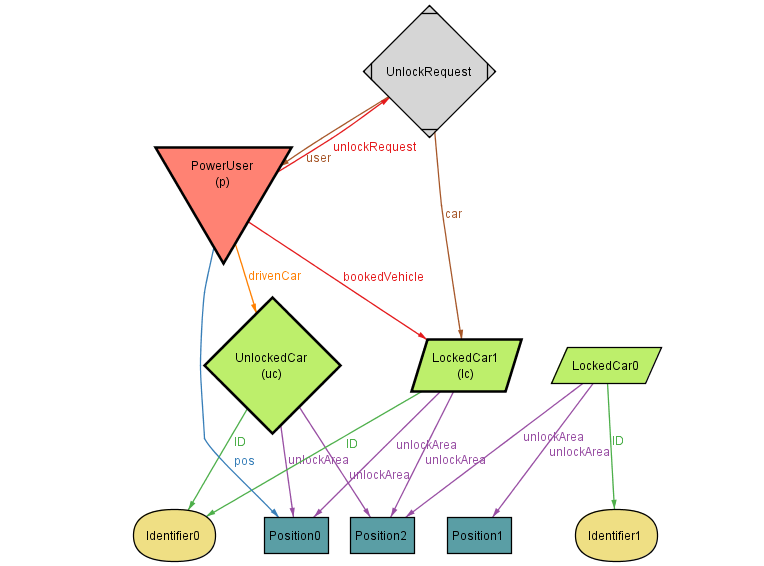
\includegraphics[scale=0.55]{{Alloy_code/unlockCar_world.png}}
    \label{fig:1Unlocking car World}
    \\Unlocking car world.
\end{figure}


\newpage

\item Cars Locking

\lstinputlisting[language=alloy]{Alloy_code/lockCars.als}


6 commands were executed. The results are:\newline
   -1: Instance found.turnOff is consistent.\newline
   -2: Instance found.lockCar is consistent.\newline
   -3: Instance found.show is consistent.\newline
   -4: No counterexample found. UnlockedCarIsTheLockedOne may be valid.\newline
   -5: No counterexample found. LockedCarStatus may be valid.\newline
   -6: No counterexample found. UnlockedCarWithEngineOffStatus may be valid.

   
\newpage

\begin{figure}[h!]
    \centering
        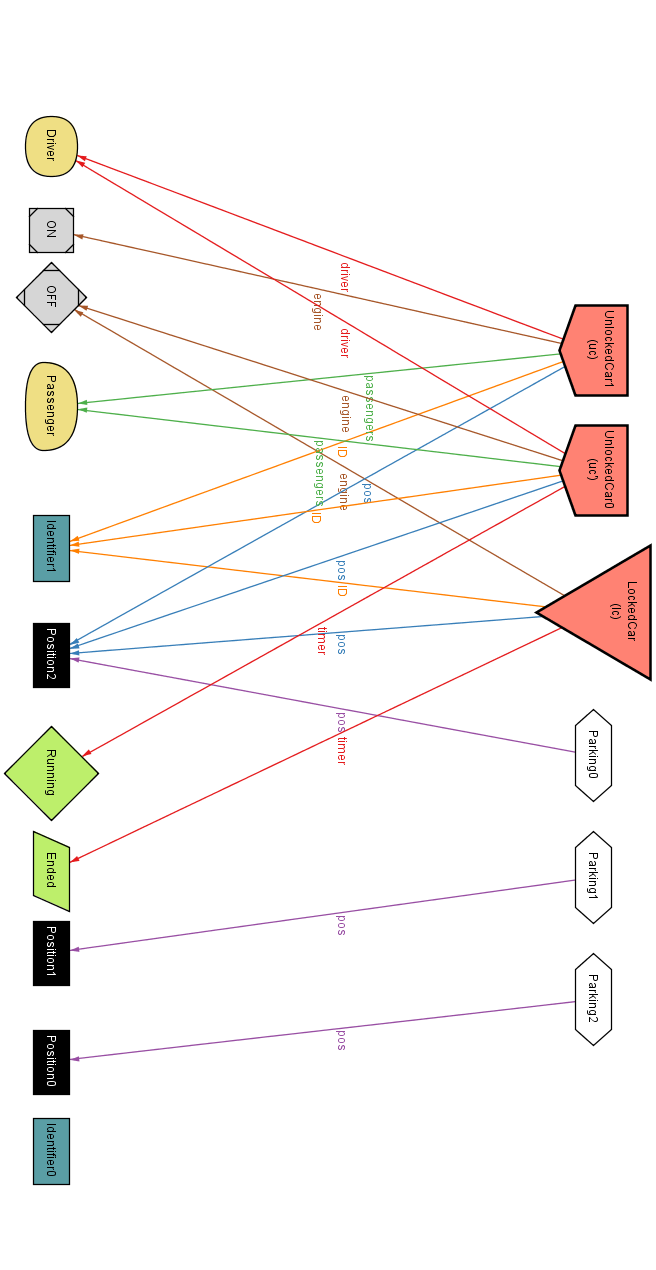
\includegraphics[scale=0.4]{{Alloy_code/lockCar_world.png}}
    \label{fig:2Locking Car World}
    \\Locking car world.
\end{figure}

\newpage
   
\item Money Saving Option 

\lstinputlisting[language=alloy]{Alloy_code/msaving_v3.als}   

2 commands were executed. The results are:\newline
   -1: Instance found.getAlternative is consistent.\newline
   -2: No counterexample found. ClosestAreaIsReachableAndFree may be valid.
   
\newpage

\begin{figure}[h!]
    \centering
        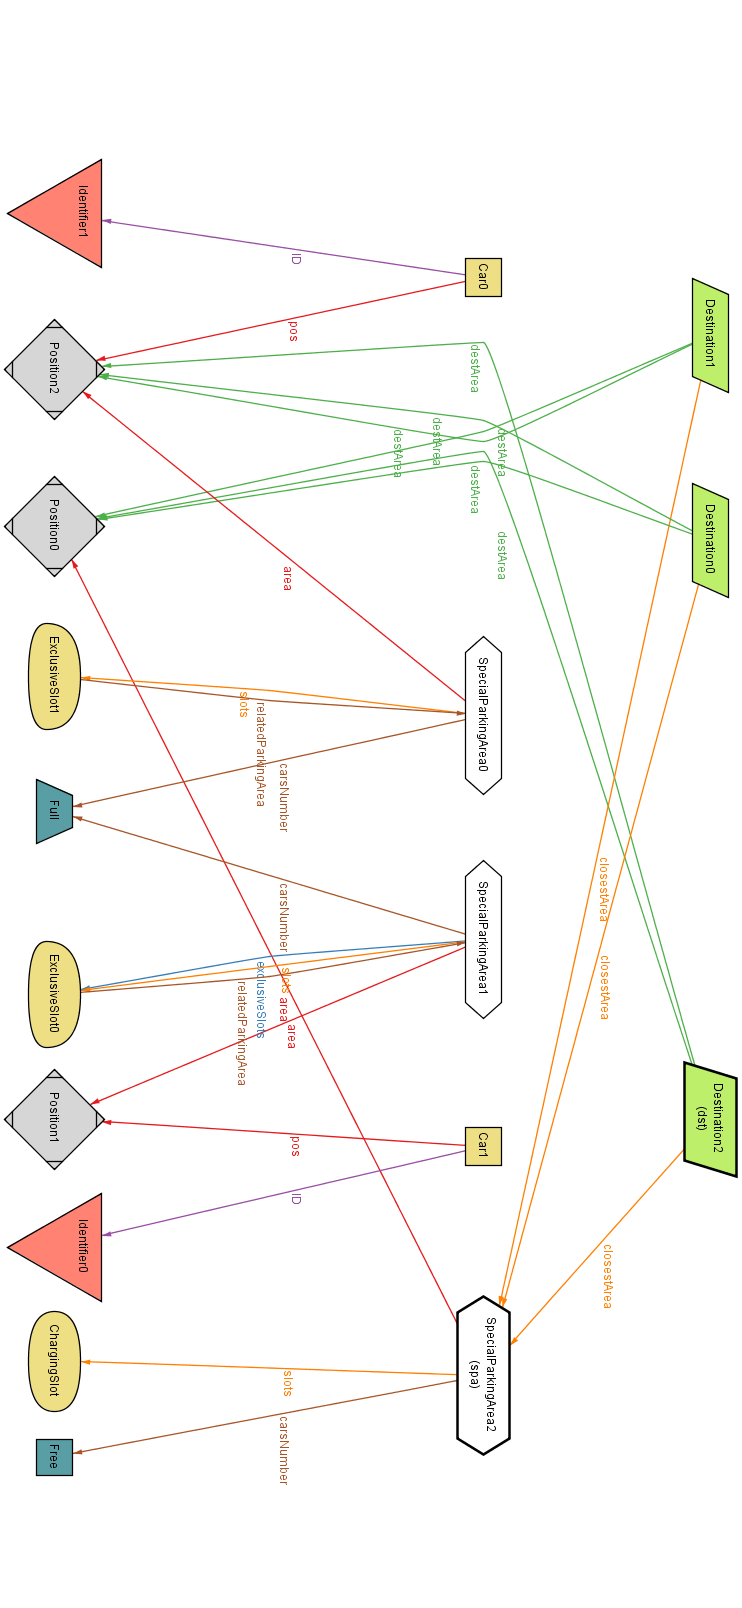
\includegraphics[scale=0.35]{{Alloy_code/msaving_world.png}} 
    \label{fig:3Money Saving World}
    \\Money saving option world.
\end{figure} 
   
\end{itemize}

\newpage
\subsection{Document revisions history}
\begin{tabular}{| l | l | p{10cm} |}
\hline
\textbf{Version} & \textbf{Date} & \textbf{Changes}\\
\hline
1.0-RC1 & 13/11/2016 & First deadline release.\\
\hline
1.0-RC2 & 11/12/2016 & Added:\newline
    - \textit{navigator} actor added in use case 4.3.10.\newline
    - definition of \textit{extends} added in the use case diagram.\newline
    - original source document of the \textit{extends} definition added in the reference section.\newline
    - figure number added to each mockup.\newline
Fixed:\newline
    - typo in Output Conditions of use case 4.3.7 fixed.\newline
    - \textit{th} added in the date on the 1\textsuperscript{st} page.\newline
    - title of subsection 5.4 updated to be consistent across all documents of the project.\newline
    - description of the figure 15 fixed.\newline
    - typo in the description of the figure 16 fixed.\\
\hline
\end{tabular} 


\subsection{Effort Spent}
\begin{tabular}{| p{5cm} | p{5cm} |}
\hline
Teamwork & $\sim$22h\\
\hline
Luca Piccirillo & $\sim$25h\\
\hline
Zampogna Gian Luca & $\sim$25h\\
\hline
Zini Edoardo & $\sim$29h\\
\hline
\end{tabular}